\documentclass[12pt,a4paper]{report}

\usepackage[utf8]{inputenc}
\usepackage[T1]{fontenc}
\usepackage[english]{babel}
\usepackage{graphicx}
\usepackage{geometry}
\usepackage{hyperref}
\usepackage{titlesec}
\usepackage{fancyhdr}
\usepackage{listings}
\usepackage{xcolor}
\usepackage{float}
\usepackage{caption}

\geometry{a4paper, margin=2.5cm}

\hypersetup{
    colorlinks=true,
    linkcolor=blue,
    filecolor=magenta,      
    urlcolor=cyan,
}

\definecolor{codegreen}{rgb}{0,0.6,0}
\definecolor{codegray}{rgb}{0.5,0.5,0.5}
\definecolor{codepurple}{rgb}{0.58,0,0.82}
\definecolor{backcolour}{rgb}{0.95,0.95,0.92}

\lstdefinestyle{mystyle}{
    backgroundcolor=\color{backcolour},   
    commentstyle=\color{codegreen},
    keywordstyle=\color{magenta},
    numberstyle=\tiny\color{codegray},
    stringstyle=\color{codepurple},
    basicstyle=\ttfamily\footnotesize,
    breakatwhitespace=false,         
    breaklines=true,                 
    captionpos=b,                    
    keepspaces=true,                 
    numbers=left,                    
    numbersep=5pt,                  
    showspaces=false,                
    showstringspaces=false,
    showtabs=false,                  
    tabsize=2
}

\lstset{style=mystyle}

\titleformat{\chapter}[display]
  {\normalfont\bfseries\huge}
  {\filleft\Large\chaptertitlename\ \thechapter}
  {1ex}
  {\titlerule\vspace{1ex}\filleft}

\newcommand{\hr}[1]{\rule{\linewidth}{#1}}

% Disable hyphenation (word division)
\hyphenpenalty=10000
\exhyphenpenalty=10000
\sloppy

\pagestyle{fancy}
\setlength{\headheight}{14.5pt}
\addtolength{\topmargin}{-2.5pt}
\fancyhf{}
\rhead{TrainingMS}
\lhead{Rapport de Projet}
\cfoot{\thepage}


\begin{document}

% --- Cover Page ---
\begin{titlepage}
    \centering
    \begin{minipage}[c]{0.2\columnwidth}
        
\includegraphics[width=\textwidth]{Figures/LogoISI.png}
    \end{minipage}
    \hfill
    \begin{minipage}[c]{0.55\columnwidth}
        \centering
        \small
        \textbf{\textsc{Republic of Tunisia}}\\
        \textbf{\textsc{Ministry of Higher Education and Scientific Research}}\\
        \textbf{\textsc{University of Tunis El Manar}}\\
        \textbf{\textsc{Higher Institute of Computer Science}}
    \end{minipage}
    \hfill
    \begin{minipage}[c]{0.2\columnwidth}
        
\includegraphics[width=0.8\textwidth]{Figures/logoutm.jpg}
    \end{minipage}
    
    \vspace{3cm}

    \rule{\linewidth}{1pt}
    \vspace{0.4cm}
    {\huge \bfseries Design and Development of a \\ Training Management System}\\[0.6cm]
    \rule{\linewidth}{1pt}
    
    \vspace{2.5cm}

    % --- Stacked Centered Authors ---
    {\large \emph{Prepared by:}} \\
    \vspace{0.4cm}
    {\Large \textbf{Firas Kahlaoui}} \\
    \vspace{0.3cm}
    {\Large \textbf{Ahmed Chaabane}} \\
    \vspace{0.3cm}
    {\Large \textbf{Seifdine Ben Fradj}} \\
    
    \vspace{1.5cm}
    
    {\large \emph{Project Type:}} \\
    \vspace{0.3cm}
    {\Large \textbf{Cas 3: Spring Boot \& React}}

    \vfill
    
    \rule{0.3\linewidth}{0.5pt}\\
    \vspace{0.2cm}
    {\large Academic Year: \textbf{2025/2026}}
\end{titlepage}

% --- Abstract ---
\chapter*{Abstract}
This project focuses on the design and development of a web-based training management system intended to improve the organization, monitoring, and evaluation of professional training activities. The existing approach relies on manual processes using paper documents and spreadsheet tools, which leads to inefficiencies, redundancy, and data inconsistency. The proposed system introduces a centralized platform that allows users to manage training sessions, participants, and trainers in a structured and reliable way. It also provides a statistical analysis module to support decision-making. The implementation of this system reduces administrative workload, improves data accuracy, and enhances the overall efficiency of training management.

\tableofcontents

\chapter{Introduction}
\section{Background and Importance}
Professional training is essential for maintaining and improving employee competencies within an organization. It enables individuals to acquire new knowledge, adapt to technological changes, and take on greater responsibilities. For employees, it serves as a vehicle for career advancement and personal growth. For organizations, continuous training leads to improved productivity, better service quality, and stronger employee engagement, ultimately contributing to a competitive advantage in a rapidly evolving market.

\section{Problem Statement}
Despite its importance, many organizations still manage training activities through traditional, manual methods. The reliance on paper-based forms and static Excel spreadsheets introduces significant limitations in scalability and data management. These manual workflows are prone to human error, data duplication, and loss of information, making it extremely difficult to monitor ongoing activities and generate reliable performance indicators.

\section{Objectives}
The objective of this project is to design and implement a centralized web-based application, titled "TrainingMS", that automates the management of training activities. The system aims to:
\begin{itemize}
    \item Provide a secure platform for data entry and validation.
    \item Centralize participant, trainer, and session information.
    \item Simplify the scheduling and planning of training programs.
    \item Offer analytical tools to visualize and evaluate training outcomes through a statistics dashboard.
\end{itemize}
By digitizing these processes, the project seeks to improve operational efficiency, ensure data integrity, and support strategic decision-making for organizational stakeholders.


\chapter{Project Context and Analysis}
\section{Existing System Analysis}
The current system for managing training activities within the organization is largely manual and fragmented. The workflow typically begins with various organizational structures submitting their annual training needs using paper-based documents. These documents include specific details such as the training domain, proposed titles, and lists of potential participants with their professional profiles and departmental affiliations.

Once these needs are collected, the information is manually transcribed into separate Excel workbooks. Each year, a new file is created, which leads to significant challenges in maintaining historical records or tracking the long-term progress of individual employees.

\section{Identified Problems}
The manual process introduces several critical issues that hinder the effectiveness of the training programs:
\begin{itemize}
    \item \textbf{Time Inefficiency}: Repetitive manual data entry and cross-referencing between documents consume substantial administrative resources.
    \item \textbf{Data Inconsistency}: Without automated validation, typographical errors and inconsistent naming conventions lead to duplicate records and unreliable data.
    \item \textbf{Lack of Real-time Tracking}: Monitoring the status of a training session or the attendance of participants requires searching through multiple physical or digital files.
    \item \textbf{Analytical Difficulty}: Generating summary statistics or performance reports is a manual, error-prone task that often yields inaccurate results.
\end{itemize}

\section{Proposed Solution: TrainingMS}
To address these limitations, we propose the development of "TrainingMS", a centralized web application. This solution focuses on the digital transformation of the training workflow through:
\begin{itemize}
    \item \textbf{Centralization}: A unified database to store all information regarding trainers, participants, formations, and historical data.
    \item \textbf{Automation}: Streamlined processes for session planning, participant enrollment, and automated validation of inputs.
    \item \textbf{Reliability}: Enforcement of data integrity through a structured relational database schema.
    \item \textbf{Decision Support}: A dedicated statistics module that provides real-time visualization of training metrics, enabling managers to evaluate the impact of training investments.
\end{itemize}
This transition from manual spreadsheets to a robust web platform ensures a scalable, secure, and efficient management environment.


\chapter{Design and Modeling}
\section{Actors and Roles}
The TrainingMS system defines three distinct user profiles to ensure secure and efficient operations:
\begin{itemize}
    \item \textbf{Simple User}: An operational user responsible for the daily management of training data. Their functionalities include authentication (login/logout), management of formations (creation, editing, deletion, and viewing), participants, and trainers. They also handle assignments, such as enrolling participants and associating trainers with specific sessions.
    \item \textbf{Manager (Responsable)}: An analytical user focused on evaluation and decision-making. Unlike the Simple User, the Manager has **read-only access** to the system's core data and cannot perform any modification, creation, or deletion. Their primary focus is the statistics dashboard, where they analyze formation counts, participant data, and budget distribution through interactive charts and advanced filters.
    \item \textbf{Administrator}: A high-level actor with full control over system configuration. Administrators manage user accounts and core referential data (domains, structures, profiles). By inheritance, the Administrator has access to all functionalities of **both** the Simple User (for data management) and the Manager (for analytical overview).
\end{itemize}

\section{Functional Requirements}
The application must support the following core capabilities:
\begin{itemize}
    \item \textbf{Authentication}: Secure login and logout using JSON Web Tokens (JWT).
    \item \textbf{CRUD Operations}: Comprehensive management (Create, Read, Update, Delete) for participants, trainers, sessions, and reference tables.
    \item \textbf{Training Planning}: Ability to schedule sessions, assign trainers, and enroll participants.
    \item \textbf{Dashboarding}: Real-time display of aggregated statistics and trends.
\end{itemize}

\section{Non-Functional Requirements}
To ensure a professional-grade application, several non-functional aspects were prioritized:
\begin{itemize}
    \item \textbf{Security}: Implementation of role-based access control (RBAC) and password encryption.
    \item \textbf{Performance}: Optimization of database queries to handle growing datasets efficiently.
    \item \textbf{Usability}: A responsive and intuitive user interface designed to minimize the learning curve.
    \item \textbf{Data Integrity}: Strict adherence to relational constraints and input validation.
\end{itemize}

\section{UML Design}
\subsection{Use Case Diagram}
The Use Case Diagram illustrates the interactions between the identified actors and the system's functionalities. The primary use cases include "Manage Formations", "Register Participants", and "Consult Dashboard", with administrative tasks such as "Manage Users" reserved for the Admin actor.

\begin{figure}[H]
    \centering
    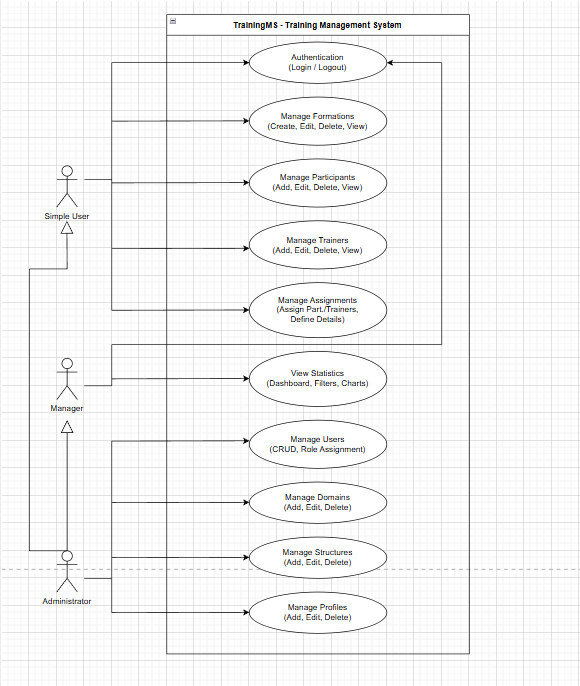
\includegraphics[width=0.8\textwidth]{Figures/Use case diagram.png}
    \caption{TrainingMS Use Case Diagram}
    \label{fig_use_case}
\end{figure}

\subsection{Class Diagram}
The core logic of the system is modeled through several interrelated entities:
\begin{itemize}
    \item \textbf{User \& Role}: Manage security and permissions.
    \item \textbf{Training Session}: The central entity representing a training session.
    \item \textbf{Participant \& Trainer}: Entities representing the human capital involved.
    \item \textbf{Domain, Structure, Profile}: Referential entities that categorize the data.
\end{itemize}
Relationships include a Many-to-Many association between \textit{Training Session} and \textit{Participant} (registrations) and Many-to-One links from \textit{Training Session} to \textit{Domain} and \textit{Trainer}.

\section{Database Design}
The relational schema was designed in MySQL to ensure optimal storage and fast retrieval. The database includes:
\begin{itemize}
    \item \textbf{Tables with Primary Keys}: All tables use auto-incremented integers as unique identifiers.
    \item \textbf{Foreign Key Constraints}: Relationships are enforced through foreign keys (e.g., \textit{idDomain} in the \textit{training session} table).
    \item \textbf{Integrity Rules}: Cascade operations and nullability constraints are defined to prevent orphaned records.
\end{itemize}
This structured approach guarantees that the data remains consistent throughout the application's lifecycle.


\chapter{Implementation and Technologies}
\section{Technology Stack}
The application is built using a modern full-stack architecture to ensure scalability and ease of maintenance:
\begin{itemize}
    \item \textbf{Backend (Spring Boot)}: Chosen for its robust security features, dependency injection, and mature ecosystem. It handles the RESTful API and business logic.
    \item \textbf{Frontend (React)}: A component-based library used to build a dynamic and responsive single-page application (SPA).
    \item \textbf{Database (MySQL)}: A reliable relational database management system used to store the structured data of the project.
\end{itemize}

\begin{figure}[H]
    \centering
    
\includegraphics[width=0.15\textwidth]{Figures/Spring-Boot-Logo.png} \hspace{1cm}
    
\includegraphics[width=0.15\textwidth]{Figures/react.png} \hspace{1cm}
    
\includegraphics[width=0.15\textwidth]{Figures/MySQL-Logo.png}
    \caption{Project Technology Stack}
    \label{fig_tech_stack}
\end{figure}

\section{System Architecture}
The backend follows a layered architecture consisting of:
\begin{itemize}
    \item \textbf{Controller Layer}: Exposes REST endpoints to the frontend.
    \item \textbf{Service Layer}: Implements the core business logic and validations.
    \item \textbf{Repository Layer}: Interface with the database using Spring Data JPA.
\end{itemize}
Security is managed via a custom filter that intercept requests to validate JWT signatures, ensuring that only authenticated users with appropriate roles can access specific resources.

\section{User Interface Design}
The user interface is designed with a focus on productivity. It features a persistent sidebar for navigation, comprehensive data tables with search and pagination capabilities, and modal-based forms for data entry. The responsive layout ensures that the system remains accessible across different device types.

\section{Statistics Module}
A critical component of TrainingMS is the statistics dashboard. It provides interactive charts (Bar, Pie, and Line charts) that visualize data such as:
\begin{itemize}
    \item Training distribution by domain.
    \item Evolution of training sessions over time.
    \item Budget utilization by organizational structure.
\end{itemize}
The module supports real-time filtering by year, domain, and trainer type. All financial data is formatted in Tunisian Dinars (TND) for local context. The dashboard automatically updates as filters are applied, providing managers with an accurate and instantaneous overview of the training landscape.


\chapter{Testing and Results}
\section{Testing Strategy}
To ensure the reliability of the application, a multi-phased testing approach was adopted:
\begin{itemize}
    \item \textbf{Functional Testing}: Each feature (e.g., creating a formation, registering a participant) was tested against its functional requirements to ensure correctness.
    \item \textbf{Validation Checks}: Input fields were tested for edge cases, including empty values, incorrect formats (e.g., invalid emails), and numeric range violations.
    \item \textbf{API Testing}: Backend endpoints were validated using tools like Postman to verify status codes, JSON response structures, and security constraints.
\end{itemize}

\section{Results and Discussion}
The development of TrainingMS successfully transitioned the organization's training management from a fragmented manual process to a centralized digital platform. 

\subsection{Improvements Over Manual System}
The primary achievements include:
\begin{itemize}
    \item \textbf{Data Accuracy}: Centralized storage eliminated the data duplication issues inherent in yearly Excel files.
    \item \textbf{Efficiency}: Search and retrieval times for participant records and session history were reduced from minutes to seconds.
    \item \textbf{Visibility}: The statistics module provided insights into training trends that were previously impossible to generate manually.
\end{itemize}

\subsection{Strengths and Limitations}
The application's strengths lie in its modular architecture and user-centric design. However, some limitations remain, such as the current lack of a mobile-specific interface and the absence of an automated email notification system for participants. These areas provide opportunities for future enhancements.


\chapter{Conclusion and Future Work}
\section{Conclusion}
This project involved the design and development of a "Training Management System" (TrainingMS) to modernize and automate the management of professional training activities. By replacing manual paper and spreadsheet-based processes with a centralized web application, the project addressed critical issues such as data inconsistency, time inefficiency, and the lack of analytical tracking. 

The successful implementation of features like role-based access control, CRUD management of entities, and an interactive statistics dashboard demonstrates the value of the platform in improving organizational productivity and data reliability. The project served as a comprehensive exercise in full-stack development, integrating Spring Boot, React, and MySQL into a coherent and functional solution.

\section{Future Work}
While the current version of TrainingMS fulfills the core requirements, several areas for future development have been identified:
\begin{itemize}
    \item \textbf{Advanced Analytics}: Integrating machine learning models to predict future training needs based on employee performance data.
    \item \textbf{Automated Notifications}: Developing a notification engine to send automated reminders and certificates via email or SMS.
    \item \textbf{Mobile Application}: Creating a dedicated mobile version for participants to view their training history and upcoming sessions on the go.
    \item \textbf{Feedback System}: Implementing an evaluation module to collect and analyze participant feedback after each session.
\end{itemize}
These enhancements will further solidify TrainingMS as a comprehensive tool for workforce development and organizational growth.


\end{document}
